As part of the design guidelines for Google Glass, Google provides developers with a card layout template, seen in Figure~\ref{GlassDesignStyle}. The different coloured regions are intended for different use. The red area is the main area intended for presenting information in text form with the green squares representing the preferred margins. The thick blue stripe almost at the bottom marks the footer. In the footer supplementary information, such as a user name or a timestamp. The blue,  slightly transparent, area to the left is mainly intended for images with associated text being presented to the right. The grey area, seemingly appearing behind all the other coloured areas, represent the entire card, with a size of 640 pixels wide and 360 pixels high~\cite{glassDesignStyle}.

	\begin{figure}[ht!]
		\centering
		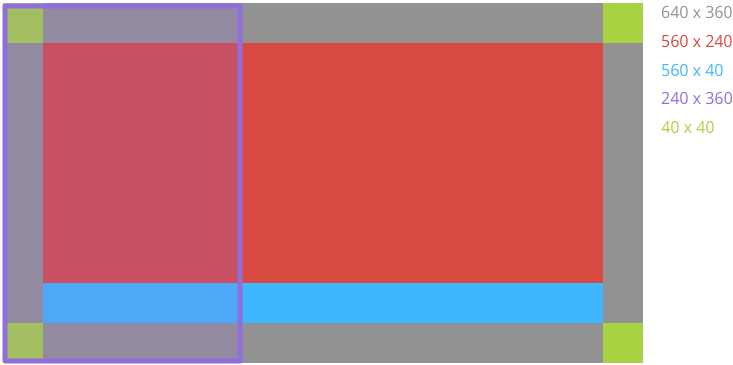
\includegraphics[width=110mm]{images/standard-template}
		\caption{Google's design guidelines include a card layout template~\cite{glassDesignStyle}.}
		\label{GlassDesignStyle}
	\end{figure}

TODO REWRITE
Google goes even further in providing developers with guidelines for design of cards. Google provides developers with a set API to use which sets up the necessary margins and everything. All the developers need to do is to input the desiered information and its ready to go. Four examples of this can be seen in Figure~\ref{cardLayouts}.

	\begin{figure}[ht!]
		\centering
   		\subfloat[Text layout.]{{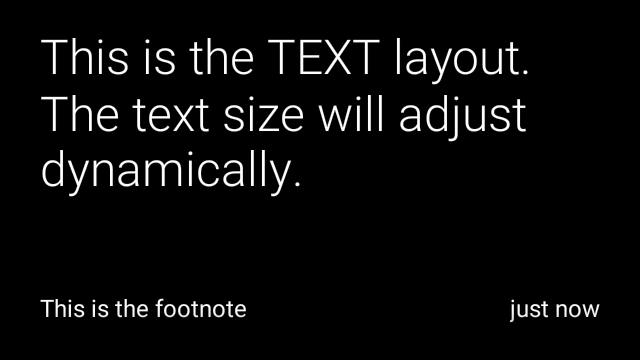
\includegraphics[width=70mm]{images/card_text} }}
  	 \qquad
   		\subfloat[Fixed text layout.]{{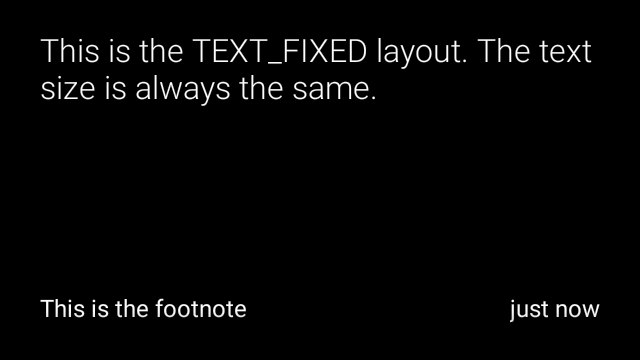
\includegraphics[width=70mm]{images/card_text_fixed} }}
	\qquad
		\subfloat[Column layout.]{{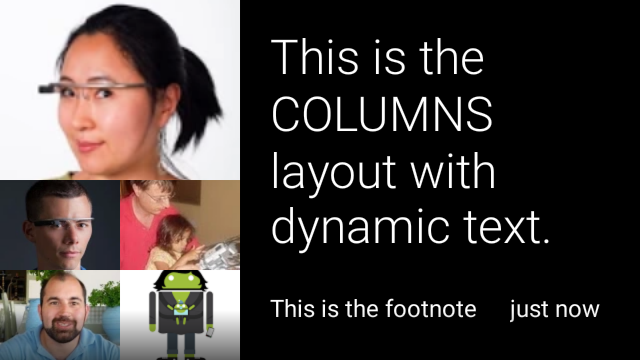
\includegraphics[width=70mm]{images/card_columns} }}
   	\qquad
		\subfloat[Title layout.]{{
\includegraphics[width=70mm]{images/card_title} }}
   	\qquad
		\caption{TODO~\cite{cardLayout}.}
		\label{cardLayouts}
	\end{figure}


[TODO Design guidelines Google Glass]

Margins layout templates

Text, Font

Google Glass Design tool

Keep it relevant  - shopping list

\begin{itemize}
\item{1}
\end{itemize}

The principles behind designing for glass is to keep the information relevant. Google ranks different computational devices and services in terms of time periods. Google talks about how the cloud stores information ``forever'', a computer keeps about a years worth of information, a mobile phone is keeping track of the last month and Glass are for the present.

Therefore Google asks developers to keep the information relevant and simple. Glass is designed not to get in the way of the user and, as stated previously, be usable when the users wants to~\cite{glassDesignPrinciples}.



Despite the fact that the display for Google Glass is placed close to the user's eye the amount of information that can be displayed is still very limited. Google have as a result provided developers with a few guidelines when writing text which will be presented on Glass~\cite{glassDesignStyle}. These guidelines, five in total, reads...

\begin{itemize}
	\item \textbf{Keep it brief.} Be concise, simple and precise. Look for alternatives to long text such as reading the content aloud, showing images or video, or removing features.
	\item \textbf{Keep it simple.} Pretend you're speaking to someone who's smart and competent, but doesn't know technical jargon and may not speak English very well. Use short words, active verbs, and common nouns.
	\item \textbf{Be friendly.} Use contractions. Talk directly to the reader using second person ("you"). If your text doesn't read the way you'd say it in casual conversation, it's probably not the way you should write it.
	\item \textbf{Put the most important thing first.} The first two words (around 11 characters, including spaces) should include at least a taste of the most important information in the string. If they don't, start over. Describe only what's necessary, and no more. Don't try to explain subtle differences. They will be lost on most users.
	\item \textbf{Avoid repetition.} If a significant term gets repeated within a screen or block of text, find a way to use it just once.
\end{itemize}

\subsubsection{Glassware Flow Designer}
Google also provides developers with a design tool to help them visualise applications prior to implementation. The design tool, called ``Glassware Flow Designer''~\cite{glasswareFlowDesigner}, allows developers to discover recommended design patterns and to see the flow of the application prior to implementation.

	\begin{figure}[ht!]
		\centering
		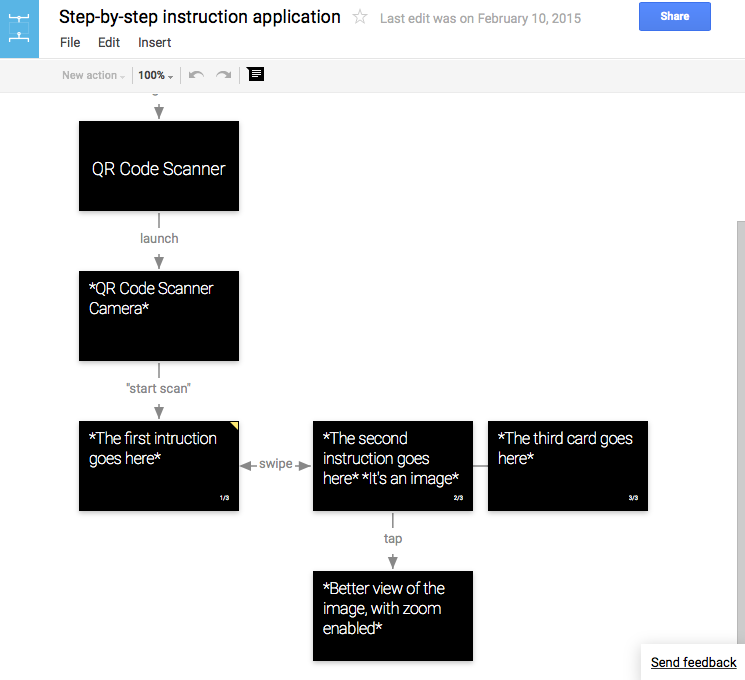
\includegraphics[width=110mm]{images/glaswareFlowDesignerScreenshot}
		\caption{The Google Glass Flow Designer.}
		\label{GlassDesignStyle}
	\end{figure}